\documentclass[12pt]{article}

\usepackage{fullpage}
\usepackage[cm-default]{fontspec}
\usepackage{xgreek}
\usepackage{float}
\usepackage{xunicode}
\usepackage{xltxtra}
\usepackage{algorithm}
\usepackage{algpseudocode}
\usepackage{amsmath}
\usepackage{mathtools}
\usepackage{unicode-math}
\usepackage{fontspec}
\usepackage{caption}
\usepackage{subcaption}
\usepackage{soul}

\setmainfont{CMU Serif}

\title{Project Ήλιος και Πλανήτης με Δορυφόρο Γραφικά Ι Χειμερινό Εξάμηνο 2016 - 2017}
\author{Χρίστος Βραχάς\\
  \texttt{sdi1300024@di.uoa.gr}
  \and Μάνος Πιτσικάλης\\
  \texttt{sdi1300143@di.uoa.gr}}
\date{}

\begin{document}

\maketitle


\section{Γενικά}

Τόσο ο ήλιος όσο και τ' αστέρια έχουν υλοποιηθεί με δύο ομόκεντρες σφαίρες, όπως προτείνεται κι από την εκφώνηση. Η θέση τους καθόριζεται μια φορά στην συνάρτηση setup.
Για τον πλανήτη και τον δορυφόρο αυτού, γίνεται parsing του αρχείου planet.obj, και δημιουργείται το αντίστοιχο μοντέλο, με βάση το οποίο στη συνέχεια
κατασκευάζεται τόσο ο πλανήτης όσο κι ο δορυφόρος. Ο πλανήτης περιστρέφεται γύρω από τον ήλιο, γύρω απο τον ίδιο, και ο δορυφόρος γύρω από τον πλανήτη. Σε κάθε επανάληψη ξαναυπολογίζονται οι θέσεις των αντικειμένων συμφώνα με τις αλλάγες που προεκυψάν από το animation αλλά και από τις επιλογές τους χρήστη.

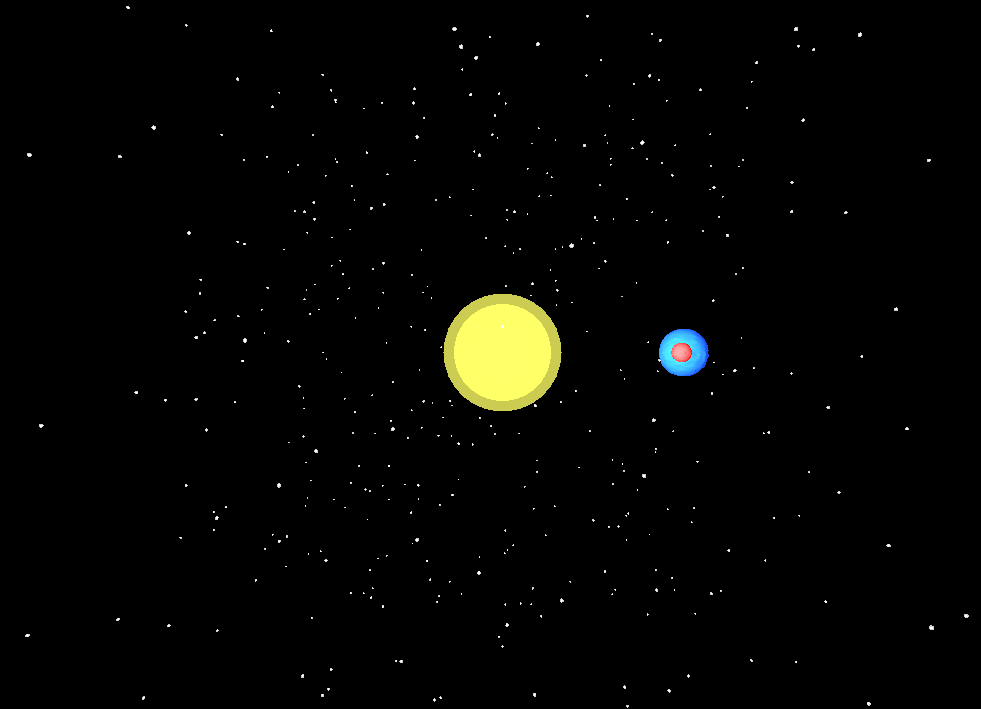
\includegraphics[scale=0.5]{graphics.png}

\section{Χειρισμός}

\begin{itemize}
    \item Παύση/Έναρξη animation : πλήκτρο p
    \item Κίνηση κάμερας : πλήκτρα w/a/s/d
    \item Τερματισμός : πλήκτρο q
\end{itemize}

\section{Περιβάλλον υλοποίησης}

Η ανάπτυξη πραγματοποιήθηκε σε περιβάλλον Linux

\end{document}
